\documentclass{article}

\usepackage{graphicx}
\usepackage{tikz}
\usepackage{tikzsymbols}
\usetikzlibrary{calc,patterns,shapes.geometric}
\pagestyle{empty}
\usepackage[margin=0pt]{geometry}
\geometry{papersize={14in,12in}}

\def\centerarc[#1](#2)(#3:#4:#5){\draw[#1] ($(#2)+({#5*cos(#3)},{#5*sin(#3)})$) arc (#3:#4:#5);}

\begin{document}
	\begin{figure}
		\centering
		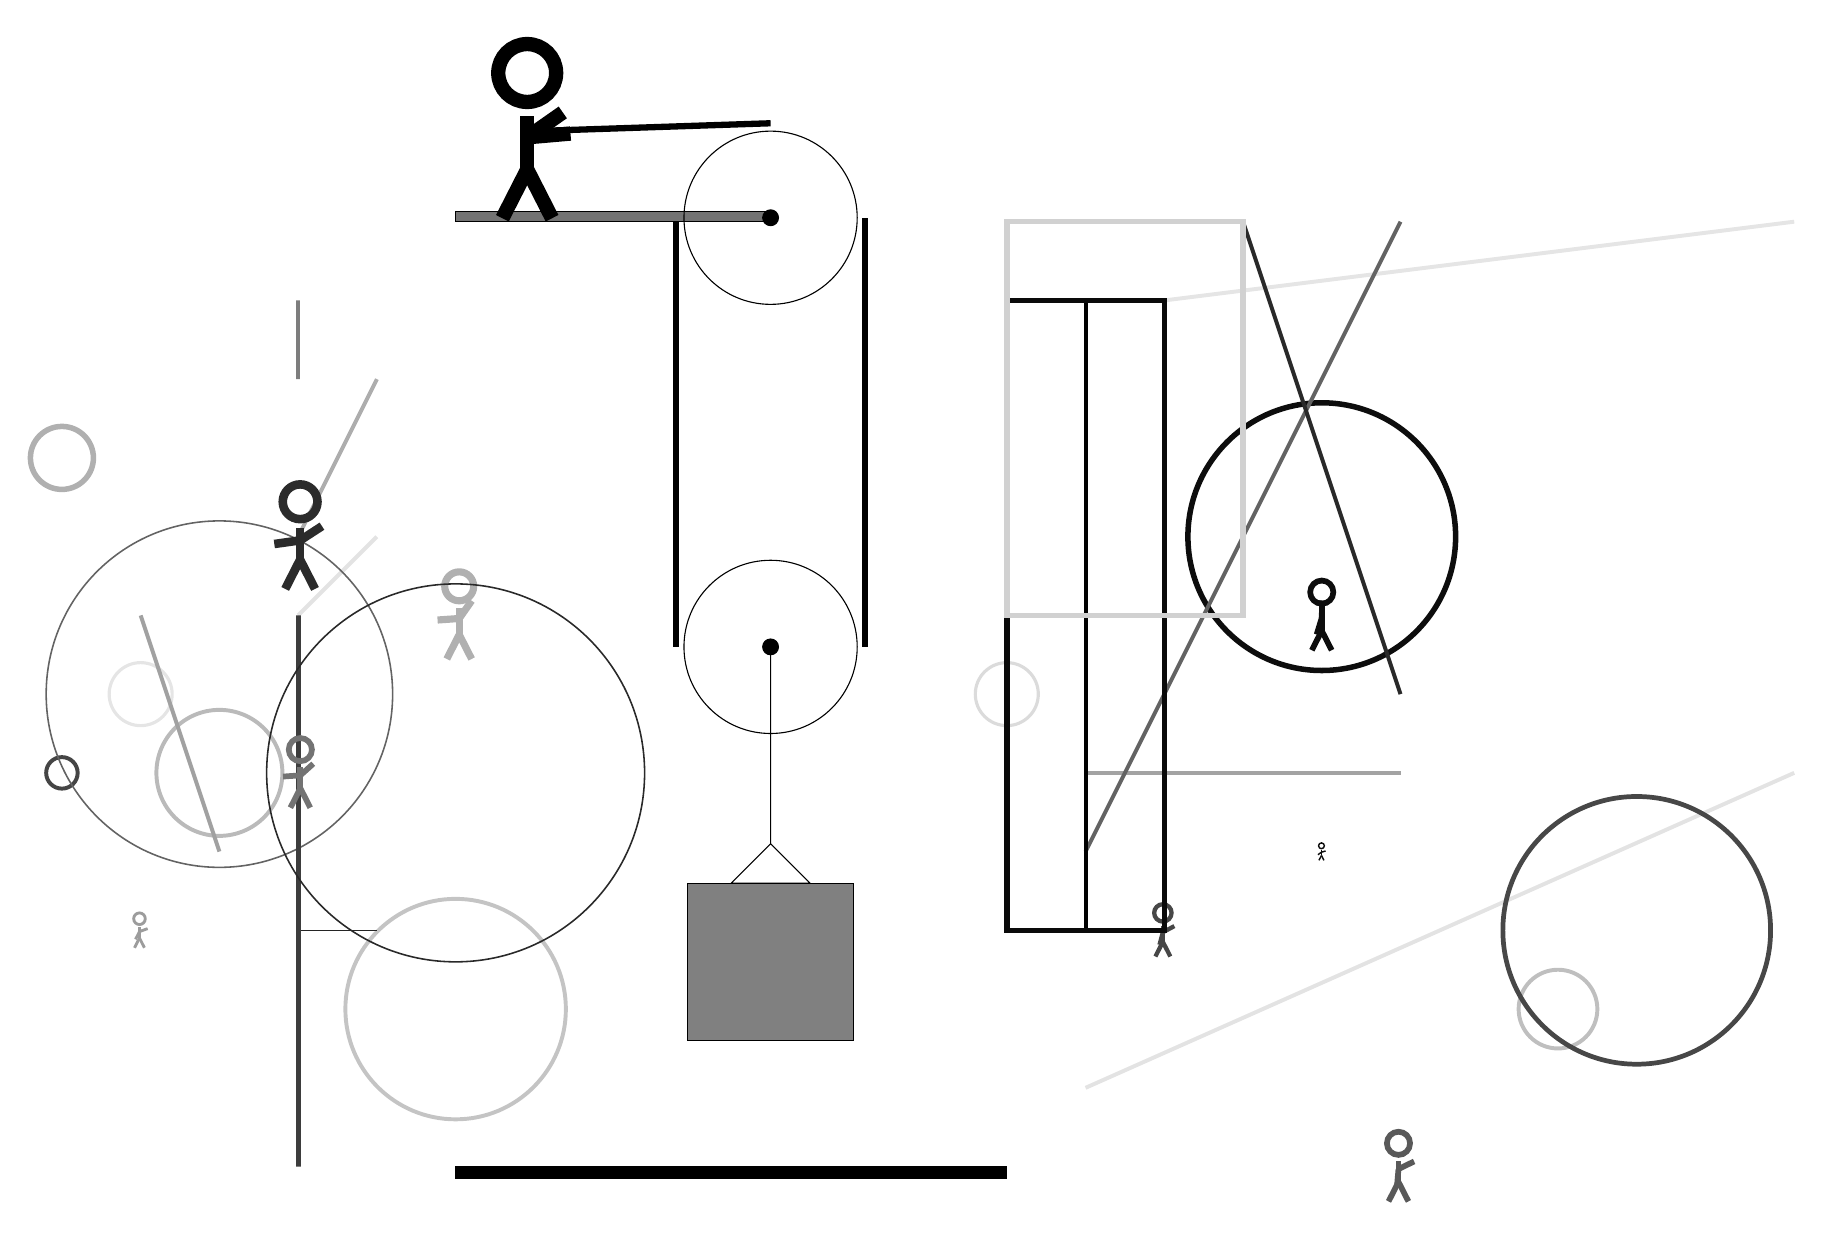
\begin{tikzpicture}
			%%%%% START %%%%%
			
			\draw[fill=black!55] (-2, 9) rectangle (2, 9.125);
			
			\draw (2, 3.6) circle (1.1);
			\draw[fill=black] (2, 3.6) circle (0.1);
			
			\draw (2, 9.05) circle (1.1);
			\draw[fill=black] (2, 9.05) circle (0.1);
			
			\draw (2, 3.6) -- (2, 1.1) -- (1.5, 0.6) -- (2.5, 0.6) -- (2, 1.1);
			\draw[fill=black!50] (0.95, 0.6) rectangle (3.05, -1.4);
			
			\draw [line width=0.5mm, color=black!23](-2, -1) circle (1.4);
			
			\draw [line width=0.5mm, color=black!27](-5, 2) circle (0.8);
			\draw [line width=0.4mm, color=black!14](5, 3) circle (0.4);
			\draw[line width=0.5mm, color=black!11](-4, 4) -- (-3, 5);
			
			\node[line width=0.6mm, color=black!95] at (9, 4) {\Strichmaxerl[4][73][89]};
			
			\node[line width=0.7mm, color=black!39] at (-6, 0) {\Strichmaxerl[2][63][20]};
			
			\draw [line width=0.5mm, color=black!73](-7, 2) circle (0.2);
			\draw [line width=0.7mm, color=black!31](-7, 6) circle (0.4);
			\draw [line width=0.7mm, color=black!95](9, 5) circle (1.7);
			
			\draw [line width=0.2mm, color=black!61](-5, 3) circle (2.2);
			\draw[line width=0.5mm, color=black!10](7, 8) -- (15, 9);
			
			\draw[line width=0.5mm, color=black!11](6, -2) -- (15, 2);
			\node[line width=0.5mm, color=black!72] at (7, 0) {\Strichmaxerl[3][75][28]};
			
			\node[line width=0.2mm, color=black!95] at (9, 1) {\Strichmaxerl[1][35][17]};
			\draw[line width=0.2mm, color=black!86] (-3, 0) rectangle (-4, 0);
			\draw[line width=0.5mm, color=black!36](10, 2) -- (6, 2);
			
			\draw [line width=0.5mm, color=black!25](12, -1) circle (0.5);
			\node[line width=0.2mm, color=black!65] at (10, -3) {\Strichmaxerl[4][85][26]};
			\draw [line width=0.6mm, color=black!72](13, 0) circle (1.7);
			
			\draw[line width=0.5mm, color=black!32](-3, 7) -- (-4, 5);
			\draw [line width=0.4mm, color=black!10](-6, 3) circle (0.4);
			
			\draw[line width=0.5mm, color=black!61](10, 9) -- (6, 1);
			
			\draw[line width=0.5mm, color=black!51] (-4, 7) rectangle (-4, 8);
			\node[line width=0.4mm, color=black!31] at (-2, 4) {\Strichmaxerl[5][4][55]};
			\draw[line width=0.6mm, color=black!76] (-4, -3) rectangle (-4, 4);
			
			\draw[line width=0.5mm, color=black!84](10, 3) -- (8, 9);
			\draw[line width=0.5mm, color=black!100] (7, 0) rectangle (6, 8);
			\node[line width=0.6mm, color=black!83] at (-4, 5) {\Strichmaxerl[6][8][33]};
			
			\draw [line width=0.2mm, color=black!84](-2, 2) circle (2.4);
			\draw[line width=0.7mm, color=black!96] (7, 0) rectangle (5, 8);
			\node[line width=0.4mm, color=black!55] at (-4, 2) {\Strichmaxerl[4][4][42]};
			
			\draw[line width=0.5mm, color=black!37](-5, 1) -- (-6, 4);
			\draw[line width=0.7mm, color=black!18] (5, 4) rectangle (8, 9);
			
			
			\draw[line width=0.8mm] (0.8, 9) -- (0.8, 3.6);
			\centerarc[line width=0.8mm](2, 3.6)(180:360:1.2000000000000002);
			\draw[line width=0.8mm](3.2, 3.6) -- (3.2, 9.05);
			\centerarc[line width=0.8mm](2, 9.05)(0:90:1.2000000000000002);
			\draw[line width=0.8mm](2, 10.25) -- (-1, 10.15);
			
			\node at (-1, 10.15) {\Strichmaxerl[10][-175][35]};
			
			\draw[fill=black] (-2, -3) rectangle (5, -3.15);
			
			%%%%% END %%%%%
		\end{tikzpicture}
	\end{figure}	
\end{document}